% Chapter 5

\chapter{IMPLEMENTATION AND RESULTS} % Write in your own chapter title

\section{Implementation}
\subsection{Identifying Computation Expressions}
\noindent
\textbf{Input}
The IR of the unoptimized code is provided as the input to the first pass of the Identifying common expression phase.\newline
\hspace{35pt}\textbf{ Output}
Annotated version of the input code is obtained, with LHS and RHS expressions marked, and the optimizable computations annotated.\newline
\textbf{Code snippet for re-associating the Expressions}

\begin{lstlisting}
void setAllMetadata(BasicBlock *BB) {
LLVMContext& context = BB->getContext();
MDBuilder builder(context);
auto *RHS = MDNode::get(context, builder.createString("RHS"));
auto *LHS = MDNode::get(context, builder.createString("LHS"));
auto *deadInst = MDNode::get(context, builder.createString(""));
...
auto onlyGEPs = getGEPs(BB);
...
\end{lstlisting}
\newpage

\subsection{Reassociating Expressions}
\noindent
\textbf{Input}\newline
The annotated IR is sent as input to the reassociating expressions pass.

\noindent
\textbf{Output}\newline
The output IR consists of the first iteration array access hoisted out of the loop. A new basic block is added to apply the predictive commoning to the loop. All the remaining instructions are marked as dead in the IR.\newline
\textbf{Code snippet for annotating the Expressions}
\begin{lstlisting}
IRBuilder<> loopBuilder(lbody, lbody->getFirstInsertionPt());
int i = 0;
for (auto it : newAllocs) {
auto newLoad = loopBuilder.CreateAlignedLoad(it, 4);
oldLoads[i]->replaceAllUsesWith(newLoad);
i++;
}
i = 0;
for (auto store: oldStores) {
auto *user = cast<Instruction>(store->getOperand(0));
IRBuilder<> tmpLoad(store->getNextNode());
tmpLoad.CreateAlignedStore(user, tmpStores[i], 4);
for (auto it = newAllocs.rbegin(); it != newAllocs.rend(); ++it) {
auto prevInst = tmpLoad.CreateAlignedLoad(*it, 4);
tmpLoad.CreateAlignedStore(prevInst, *(++it), 4);
}
auto prevInst = tmpLoad.CreateAlignedLoad(tmpStores[i], 4);
tmpLoad.CreateAlignedStore(prevInst, *newAllocs.rbegin(), 4);
i++;
}

\end{lstlisting}

\section{Modules}
\subsection{Identifying Computation Expressions}
The two modules are implemented in three passes, of which the first pass alone constitutes the first module. In the first pass, we iterate through the input IR to find the basic blocks with loops, using the \texttt	{getLoopAnalysisUsage} class. After finding the loop containing block, we iterate through the basic blocks found in that block, to find initial iteration of the loop. We define \texttt{getInitial()} function to get the initial iteration. Upon getting the initial iteration, we check for dominant and dominated expressions. If a basic block inside the loop contains both dominant and dominated load expressions, we set the metadata using the 
\texttt{setAllMetaData()} function. The \texttt{MDNode::get()} function is used to retrieve the text Metadata node needed to annotate the expresssions, using the \texttt{ setUsersMetadata(dominant, gepIT, deadInst)} function call. These steps are all iteratively done by invoking the \texttt{runOnLoop()} function. 

\subsection{Reassociating Expressions}
The second pass is run on each function, and it hoists the indexed expressions out of the loop and adds a new basic block, to add the swapping instructions at the end. On finding the loop containing blocks, we get the annotations by using the \texttt{instr->getMetadata()} function. 

By ensuring that the annotations are what we require, we create a new basic block, and also hoist the instructions out of the loop. \texttt{builder.CreateAlloca()} function is used to create a new allocation for the hoisted first iteration value. The old loads are collected, and pushed in a vector. Once the new loads with array access eliminated are construcuted, all the old loads are replaced with the new loads. 

\texttt{CreateAlignedStore} is used to create the replacing store instructions that will be used to create the swapping block at the bottom of the loop body. 

\begin{lstlisting}
IRBuilder<> loopBuilder(lbody, lbody->getFirstInsertionPt());
int i = 0;
for (auto it : newAllocs) {
auto newLoad = loopBuilder.CreateAlignedLoad(it, 4);
oldLoads[i]->replaceAllUsesWith(newLoad);
i++;
}

\end{lstlisting}
\hspace{55pt} \textbf{Replacing the instructions with IRBuilder}

\section{Removal of Dead Instructions}
Once the two initial passes are done, we eliminate the dead instructions by eliminating its uses and then removing it using the \texttt{i->eraseFromParent()} function call.


\section{Experimental Results}
The proposed optimization is used on 4 different test cases. The Relative Improvement Percentage (RIP) is the difference of optimization times between the two versions with and without applying the optimization. The optimization time is defined as the sum of both the compilation time and the running time.

\begin{equation*}
RIP \% = \frac{T_{unoptimized}-T_{optimized}}{T_{optimized}} x 100% 
\end{equation*}

If  $RIP\%$ is negative,  the  optimization has a negative effect, so it is better to not apply the optimization,

We evaluate our optimization with three different test cases which cover most use cases of our optimization

\subsection{Performance Evaluation}

\subsubsection{Test Case 1}

The Fibonacci sequence is used as the code for this test case. Traditional way of finding Fibonacci includes accessing two array indexes to calculate the successor. 

The results of applying our optimization are

\begin{figure}[H]
	%	\centering
	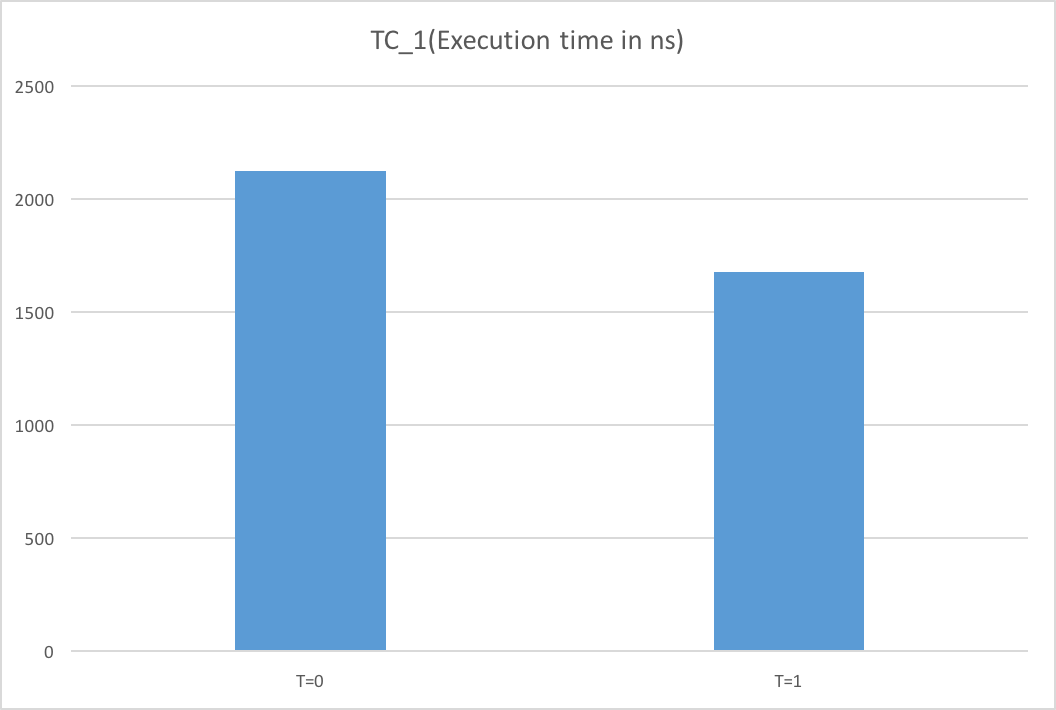
\includegraphics[scale=0.8]{tc_1.png}
	\caption{Execution times for TC 1}
	\label{TC_1}	
\end{figure}

\subsubsection{Test Case 2}

The optimization quality is proportional to the number of array accesses in the loop. This is depicted by this use case. 

The results of applying our optimization are

\begin{figure}[H]
	\centering
	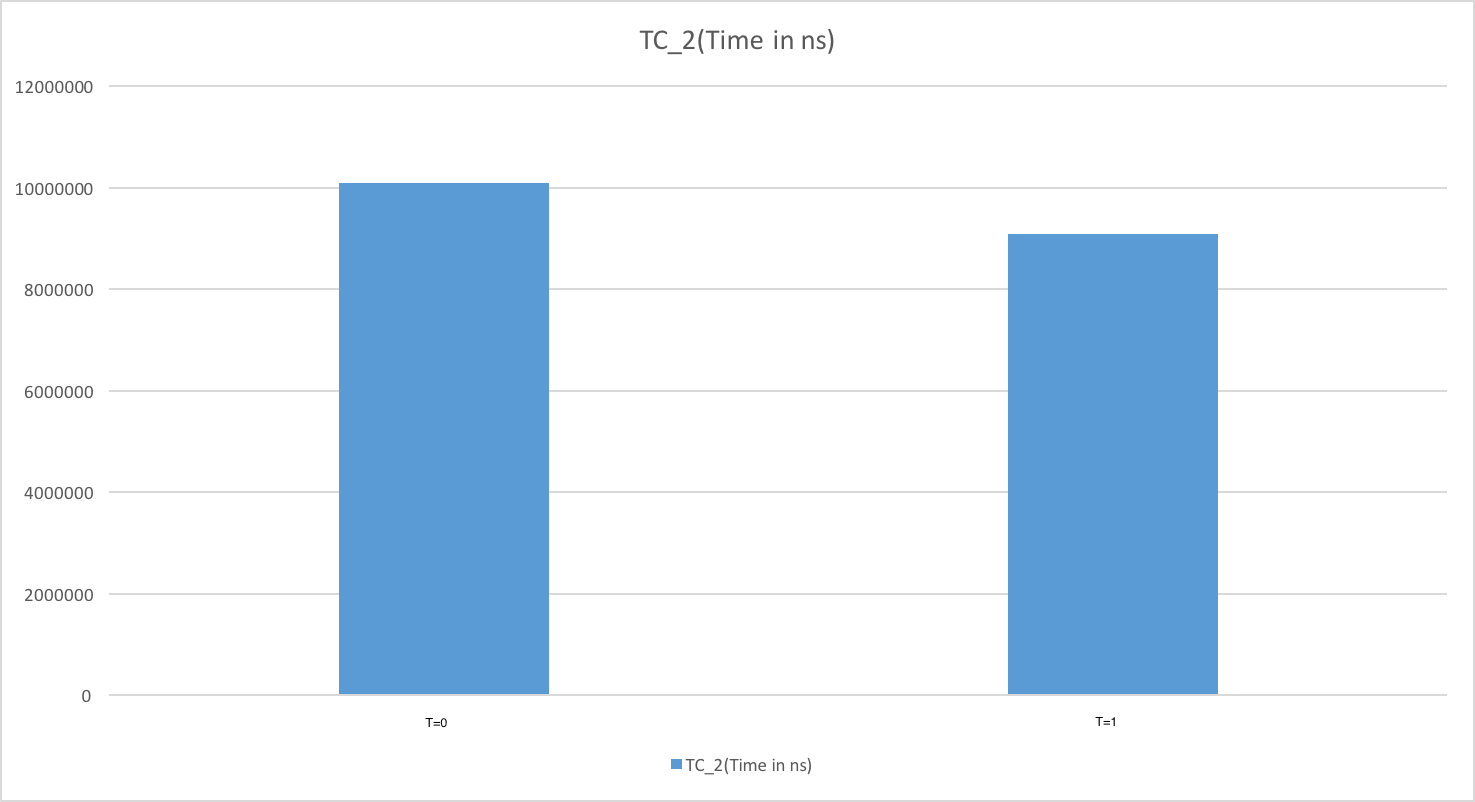
\includegraphics[scale=0.5]{tc_2.png}
	\caption{Execution times for TC 2}
	\label{TC_2}	
\end{figure}

\subsubsection{Test Case 3}

Not applying the optimization when not needed is also an evaluation of our system. Keeping this in mind, this test case contains code which cannot be optimized.

The results of applying our optimization are depicted in \ref{TC_3}

\begin{figure}[H]
	\centering
	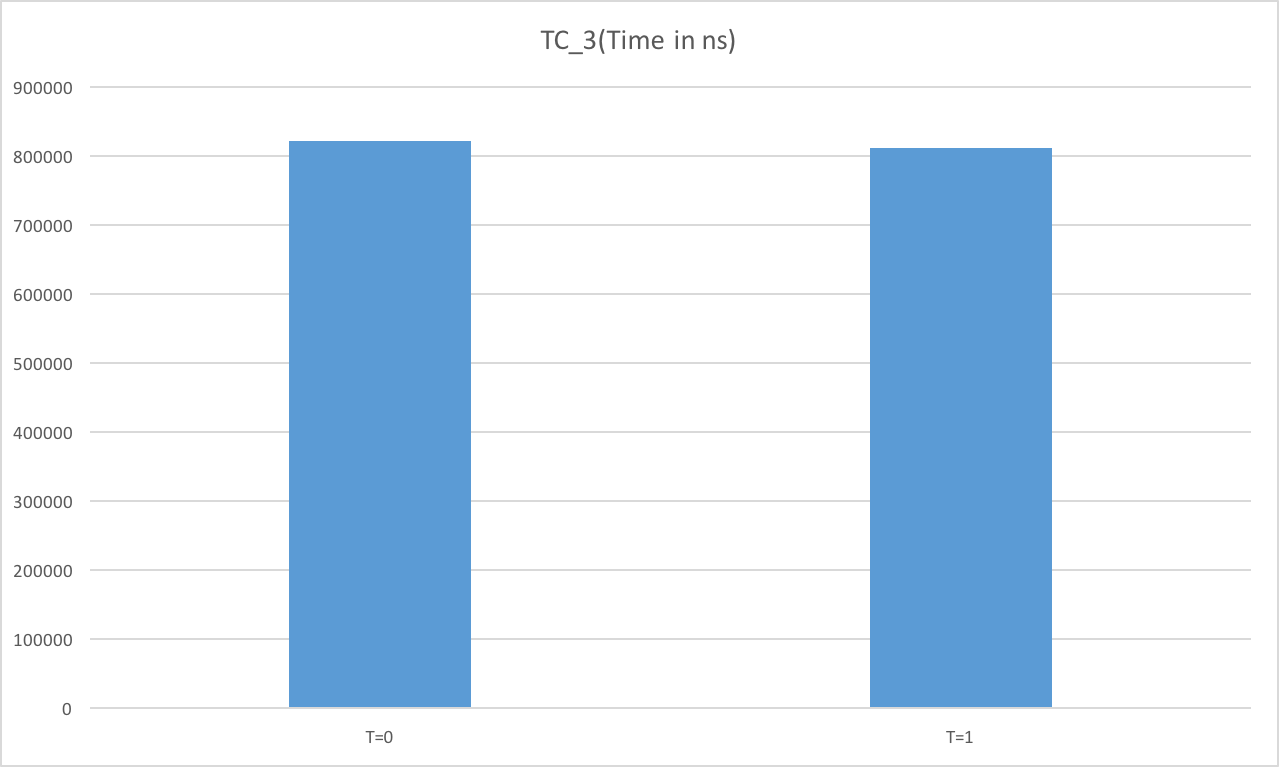
\includegraphics[scale=0.3]{tc_3.png}
	\caption{Execution times for TC 3}
	\label{TC_3}	
\end{figure}

\pagebreak

\subsection{Evaluation}

For each test case, we then find the RIP according to our formula. The results are below 

\begin{figure}[H]
	\centering
	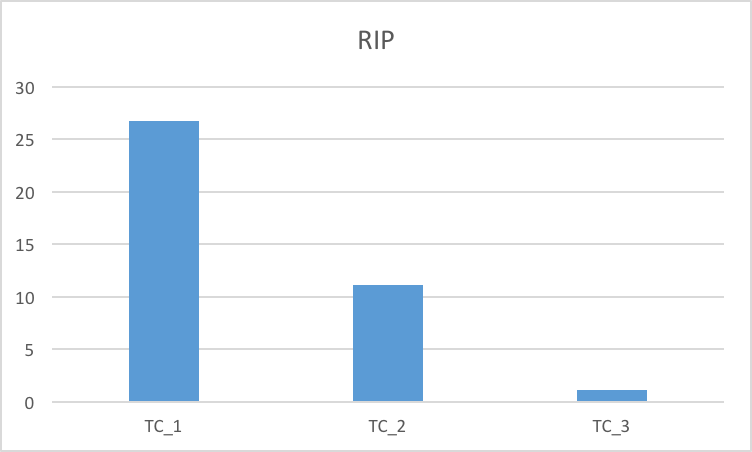
\includegraphics[scale=0.5]{rip.png}
	\caption{RIP of all test cases}
	\label{RIP}	
\end{figure}

We can deduce the following observations

\begin{enumerate}
	\item The performance is directly proportional to the number of array accesses present in the loop.
	\item There is no improvement or deterioration when the optimized is not applicable. 
\end{enumerate}
